% Protocolo aleatório com validação cruzada (Seção Protocolos de avaliação, 03-Metodologia.tex)
% Cores usadas nesta figura (valores CMYK da paleta dvipsnames do xcolor), definidas aqui para não depender de opções externas
\definecolor{RoyalBlue}{cmyk}{1,0.50,0,0}
\definecolor{BurntOrange}{cmyk}{0,0.51,1,0}
\definecolor{ForestGreen}{cmyk}{0.91,0,0.88,0.12}
\begin{figure}[htbp]
    \centering
    \caption{Protocolo aleatório: divisão 70/30 e validação cruzada dentro do treino}
    \label{fig:met-protocolo-aleatorio}
    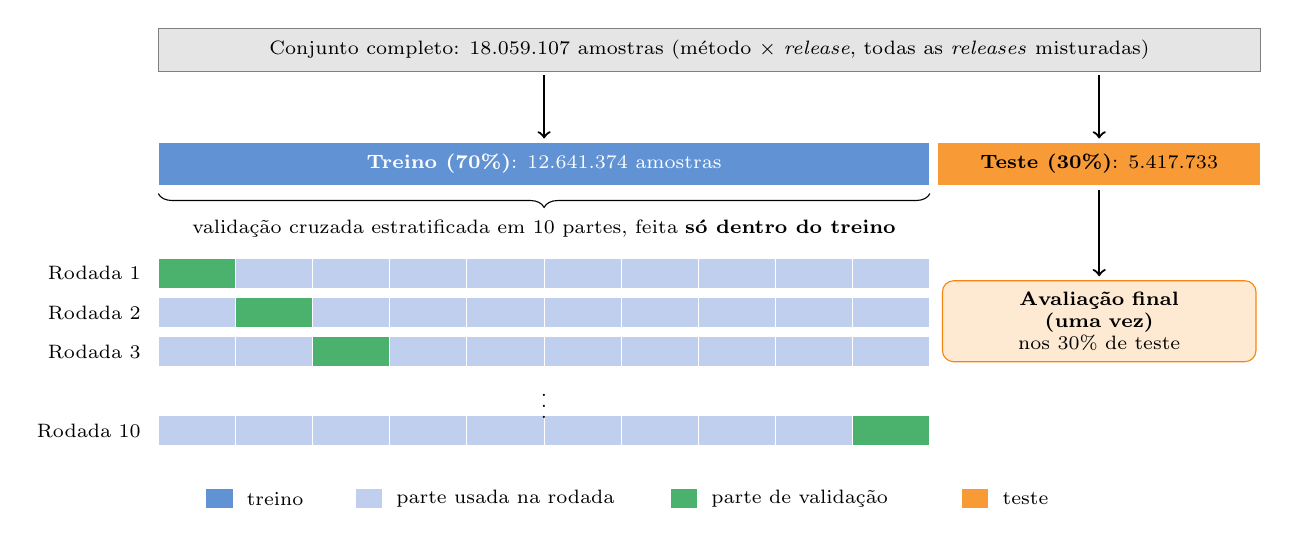
\begin{tikzpicture}[x=1cm,y=1cm,font=\scriptsize,
        caixa/.style={draw,rounded corners,align=center,inner sep=4pt},
        chave/.style={decorate,decoration={brace,amplitude=5pt,mirror}}]
        % ---- conjunto completo
        \filldraw[fill=gray!20,draw=gray] (0,0) rectangle (14,0.55);
        \node at (7,0.275) {Conjunto completo: 18.059.107 {\azul amostras} (método $\times$ \textit{release}, todas as \textit{releases} misturadas)};
        \draw[->,thick] (4.9,-0.05) -- (4.9,-0.85);
        \draw[->,thick] (11.95,-0.05) -- (11.95,-0.85);
        %\node[align=center,text=gray] at (8.4,-0.45) {divisão aleatória estratificada (semente 42):\\ 0,49\% de positivos nos dois conjuntos};
        % ---- treino e teste
        \filldraw[fill=RoyalBlue!65,draw=white] (0,-1.45) rectangle (9.8,-0.9);
        \node[text=white] at (4.9,-1.175) {\textbf{Treino (70\%)}: 12.641.374 {\azul amostras}};
        \filldraw[fill=BurntOrange!80,draw=white] (9.9,-1.45) rectangle (14,-0.9);
        \node at (11.95,-1.175) {\textbf{Teste (30\%)}: 5.417.733};
        % ---- validação cruzada (só dentro do treino)
        \draw[chave] (0,-1.55) -- (9.8,-1.55) node[midway,below=6pt]
            {validação cruzada estratificada em 10 partes, feita \textbf{só dentro do treino}};
        \foreach \k/\y/\nome in {1/-2.75/Rodada 1, 2/-3.25/Rodada 2, 3/-3.75/Rodada 3, 10/-4.75/Rodada 10}{
            \node[anchor=east] at (-0.1,{\y+0.19}) {\nome};
            \foreach \p in {1,...,10}{
                \ifnum\p=\k
                    \filldraw[fill=ForestGreen!75,draw=white] ({(\p-1)*0.98},\y) rectangle ++(0.98,0.38);
                \else
                    \filldraw[fill=RoyalBlue!25,draw=white] ({(\p-1)*0.98},\y) rectangle ++(0.98,0.38);
                \fi}}
        \node at (4.9,-4.15) {$\vdots$};
        % ---- avaliação final no teste
        \draw[->,thick] (11.95,-1.5) -- (11.95,-2.6);
        \node[caixa,fill=BurntOrange!15,draw=BurntOrange,text width=3.7cm,anchor=north] at (11.95,-2.65)
            {\textbf{Avaliação final}\\\textbf{(uma vez)}\\nos 30\% de teste};
        % ---- legenda
        \begin{scope}[shift={(0.6,-5.55)}]
            \filldraw[fill=RoyalBlue!65,draw=white] (0,0) rectangle ++(0.35,0.25);
            \node[anchor=west] at (0.4,0.125) {treino};
            \filldraw[fill=RoyalBlue!25,draw=white] (1.9,0) rectangle ++(0.35,0.25);
            \node[anchor=west] at (2.3,0.125) {parte usada na rodada};
            \filldraw[fill=ForestGreen!75,draw=white] (5.9,0) rectangle ++(0.35,0.25);
            \node[anchor=west] at (6.3,0.125) {parte de validação};
            \filldraw[fill=BurntOrange!80,draw=white] (9.6,0) rectangle ++(0.35,0.25);
            \node[anchor=west] at (10.0,0.125) {teste};
        \end{scope}
    \end{tikzpicture}
    \fonte{Elaborado pelo autor (2026).}
\end{figure}%
